\chapter{Moment of Inertia and Angular Momentum}

Why does a figure skater spin faster when pulling in their arms? Why does a hollow ball roll downhill more
slowly than a solid one? Why does a heavy flywheel keep spinning long after you stop pushing it? In the Torque
and Equilibrium chapter, you learned what makes things start to turn. This chapter is about how hard they are to
turn, and about the energy and momentum that rotating objects carry.

\section{Moment of Inertia and Rotational $F=ma$}\index{moment of inertia}
We know Newton's Second Law by heart now, $F_{net} = ma$. You probably could recite it in your sleep, but what about a rotational equivalent. Recall that from our first circular motion chapter, we have the equation $a = r \alpha$. Let us do some conversions to get this into an angular form:
\begin{align}
    F &= ma \notag \\
    F &= mr\alpha \notag \\
    rF &= mr^2\alpha \notag \\
    \tau &= mr^2\alpha \label{eq:rotNewt2ndLaw}
\end{align}

From Equation~\ref{eq:rotNewt2ndLaw}, we can derive that the ``mass equivalent'' is $mr^2$, since $m$ is multiplied by $a$ in the linear $F=ma$, while $mr^2$ is multiplied by $\alpha$. Thus, we can state that for a point of distance $r$ from the pivot (or axis of rotation), that singular point has \emph{rotation inertia}, also called \emph{moment of inertia}, is defined as $mr^2$. For a whole object, the total moment of inertia is the sum of $mr^2$ over all its pieces.
\begin{mdframed}[frametitle = {Moment of Inertia}, style = important]
    A mass's total moment of inertia is given by the sum of each mass multiplied the distance from the axis of rotation squared.
    \begin{equation}
        I = \sum m r^2\label{eq:momentInertiaSum}
    \end{equation}
    For a solid object, think of it as millions of tiny pieces and add up $mr^2$ for every one. (In calculus,
    this kind of sum becomes an \emph{integral}, which you will learn about later.)
\end{mdframed}
From Equation~\ref{eq:momentInertiaSum}, we see that mass farther from the axis matters much more than anything closer to the pivot. For two objects with the same mass and radius, one solid (mass spread evenly throughout) and the other a hollow cylinder or hoop (mass at the rim), the hollow one has the greater moment of inertia. That is part of why a figure skater spins faster after pulling their arms in: moving mass toward the axis shrinks the moment of inertia.

By finding the net rotational inertia of an object, we can create an equation for the rotational equivalent of Newton's Second Law:
\begin{equation}
    \sum \tau = \tau_{net} = I \alpha
    \label{eq:ialpha}
\end{equation}

\subsection{Relating $\tau = I \alpha$ and other Torque Def'ns}
Since we have already defined angular acceleration, and have just discussed moment of inertia, we can now relate our two torque equations, $\tau = rF\sin\theta$ from the Torque and Equilibrium chapter, and Equation~\ref{eq:ialpha} by equating them, as they both equal net torque.
\begin{equation}
  I \alpha = r F \sin\theta
  \label{eq:torqueequivs}
\end{equation}
This will be useful for solving rotational dynamics problems, and finding any of the variables $I$, $\alpha$, $r$, $F$, or $\theta$ when the others are known.
\begin{Exercise}[title=Angular Acceleration of a Wheel,label=angacc1]
A wheel has \(I=0.80\ \text{kg·m}^2\). A force \(F=25\ \text{N}\) is applied at radius \(r=0.40\ \text{m}\) at an angle \(\theta=60^\circ\) to the radius.

Find \(\alpha\).

\end{Exercise}
\begin{Answer}[ref=angacc1]
Using Equation~\ref{eq:torqueequivs}, we can rearrange to solve for $\alpha$ as $\alpha = \frac{r F \sin\theta}{I}$.
\[
\alpha = \frac{r F \sin\theta}{I} = \frac{0.40 \cdot 25 \sin60}{0.8} \approx 10.825 \text{ rad / s}^2
\]

\end{Answer}


\begin{Exercise}[title=Moment of Inertia from Multiple Torques,label=mominert1]
A rigid wheel is mounted on a frictionless axle. Two forces act on the wheel:

\begin{itemize}
\item Force $F_1 = 30\ \text{N}$ is applied at radius $r_1 = 0.50\ \text{m}$ at an angle $\theta_1 = 90^\circ$ to the radius, producing a counterclockwise torque.
\item Force $F_2 = 20\ \text{N}$ is applied at radius $r_2 = 0.30\ \text{m}$ at an angle $\theta_2 = 45^\circ$ to the radius, producing a clockwise torque.
\end{itemize}

The wheel undergoes an angular acceleration of $\alpha = 8.0\ \text{rad/s}^2$.

Find the moment of inertia $I$ of the wheel.
\end{Exercise}
\begin{Answer}[ref=mominert1]
We choose counterclockwise torques to be positive. The net torque is

\[
\sum \tau = r_1 F_1 \sin\theta_1 - r_2 F_2 \sin\theta_2
\]

Using the rotational form of Newton's second law,

\[
\sum \tau = I \alpha
\]

Solving for $I$,

\[
I = \frac{r_1 F_1 \sin\theta_1 - r_2 F_2 \sin\theta_2}{\alpha}
\]

Substituting values,

\[
I = \frac{(0.50)(30)\sin90^\circ - (0.30)(20)\sin45^\circ}{8.0}
\]

\[
I = \frac{15 - 4.24}{8.0} \approx 1.35\ \text{kg·m}^2
\]

\end{Answer}

\section{Parallel-Axis Theorem}

The \textbf{parallel-axis theorem} allows us to calculate the moment of inertia of a rigid body about any axis that is parallel to an axis passing through the center of mass. The theorem states that \index{parallel-axis theorem}
\begin{equation}
I_s = I_{cm} + Md^2
\end{equation}
where $I_s$ is the moment of inertia about the axis of interest, $I_{cm}$ is the moment of inertia about a parallel axis through the center of mass, $M$ is the total mass of the object, and $d$ is the perpendicular distance between the two axes.

In many practical situations, such as a door rotating about its hinges or a rod rotating about one end, the axis of rotation is offset from the center of mass, making direct calculation more difficult. That is where the parallel axis theorem comes in!

\begin{Exercise}[title=Parallel Axis Theorem, label=parallelAxisThm1]
Prove that the Moment of Inertia of the end of a rod is $I_{end} = \frac{1}{3}ML^2$ given that the moment of inertia of a rod about its center of mass is $I_{CM} = \frac{1}{12}ML^2$.
\end{Exercise}
\begin{Answer}[ref=parallelAxisThm1]
\begin{align*}
  I_{end} &= I_{CM} + MD^2 \\
          &= \frac{1}{12}ML^2 + M\left( \dfrac{L}{2} \right)^2\\
          &= \frac{1}{12}ML^2 + M\left( \dfrac{L^2}{4} \right) \\ 
          &= \left(  \dfrac{1}{12} + \dfrac{1}{4}  \right)ML^2 \\
          &= \left(  \dfrac{4}{12}  \right) ML^2\\
          &= \dfrac{1}{3} ML^2
\end{align*}
\end{Answer}

The parallel-axis theorem shows that the moment of inertia about an offset axis is always greater than the moment of inertia about the center-of-mass axis. The additional term $Md^2$ accounts for the translational motion of the object's center of mass relative to the new axis of rotation. As the distance between the axes increases, the moment of inertia increases accordingly.

If the mass of an object is not evenly distributed, the location of the center of mass shifts, but the parallel-axis theorem remains applicable. Once the center of mass is known, the theorem allows the moment of inertia about any parallel axis to be found by adding the contribution due to the displacement of the center of mass. In this way, the effects of mass distribution are fully captured by the center-of-mass term and the distance between the axes.


\section{Rotational Kinetic Energy and Rolling Motion}\index{rolling motion}
Take a look at this video: \href{https://www.youtube.com/watch?v=CHQOctEvtTY}{Rotational Inertia: The Race Between a Ring and a Disc}.

Let us analyze why the solid cylinder reaches the bottom first.

When two objects roll down an incline without slipping, their acceleration depends not only on gravity, but also on how their mass is distributed. This is because a rolling object must both translate and rotate, so gravitational potential energy is split between translational and rotational kinetic energy. The fraction that goes into rotation depends on the object's moment of inertia.

When an object is rolling, it has both translational kinetic energy and rotational kinetic energy. The total kinetic energy of a rolling object is the sum of these two forms of kinetic energy.

The total rotational kinetic energy of a rolling object comes from all of its individual point masses rotating around the axis. Each point mass has its own rotational kinetic energy $K_i$, and the sum of all these individual kinetic energies gives the total rotational kinetic energy of the object:
\begin{align*}
KE_{\text{rotational}}
&= \sum K_i \\
&= \sum \tfrac{1}{2} m_i r_i^2 \omega^2 \\
&= \tfrac{1}{2} \left( \sum m_i r_i^2 \right) \omega^2 \\
\end{align*}

This gives us the formula for rotational kinetic energy in terms of moment of inertia:
\begin{mdframed}[frametitle = {Rotational Kinetic Energy}, style = important]
\index{rotational kinetic energy}The rotational kinetic energy of a rigid body rotating about a fixed axis is given by
\begin{equation}
  KE_{\text{rotational}} = \tfrac{1}{2} I \omega^2
\label{eq:rotKE}
\end{equation}
where $I$ is the moment of inertia of the object about the axis of rotation, and $\omega$ is the angular velocity. This expression applies to rigid bodies rotating about a fixed axis.
\end{mdframed}

Going back to our rolling objects, we can now see that the total kinetic energy of a rolling object is the sum of its translational and rotational kinetic energies:
\begin{mdframed}[frametitle = {Total Kinetic Energy of a Rolling Object}, style = important]
The total kinetic energy of a rolling object is given by
\begin{equation}
  KE_{\text{total}} = KE_{\text{translational}} + KE_{\text{rotational}} = \tfrac{1}{2} mv^2 + \tfrac{1}{2} I \omega^2
\label{eq:totalKErolling}
\end{equation}
where $m$ is the mass of the object, $v$ is its linear velocity, $I$ is its moment of inertia, and $\omega$ is its angular velocity. For rolling without slipping, the translational and rotational motions are linked, but it is still useful to treat their kinetic energies separately.
\end{mdframed}

The moment of inertia $I$ varies depending on how the mass is distributed in the object, and is a measure of how much the object resists rotational motion. For example, a solid disc has a different moment of inertia than a hollow disc of the same mass and radius. This difference in moment of inertia affects how much of the total kinetic energy is rotational versus translational.

The solid disc has most of its mass concentrated closer to the center, resulting in a lower moment of inertia. This means that less of its total kinetic energy is rotational, allowing more energy to be available for translational motion, which leads to a higher linear velocity down the incline.

\begin{mdframed}[frametitle = {Relationship between translational velocity and moment}, style = important]
For an object of mass $m$ and radius $R$ rolling without slipping from
rest down a height $h$, $\omega = \frac{v}{R}$, so energy conservation gives
$mgh = \frac{1}{2}mv^2 + \frac{1}{2}I\frac{v^2}{R^2}$, and
\begin{equation}
v = \sqrt{\frac{2gh}{1 + \frac{I}{mR^2}}}
\end{equation}
The larger $\frac{I}{mR^2}$ is, the slower the object rolls. A solid
cylinder ($\frac{I}{mR^2} = \frac{1}{2}$) reaches $\sqrt{\frac{4}{3}gh}$,
while a hoop ($\frac{I}{mR^2} = 1$) reaches only $\sqrt{gh}$, whatever
their masses and sizes.
\end{mdframed}

Each object has a unique moment of inertia based on its mass distribution, which directly affects its rolling behavior. Here is a reference table with common moments of inertia for various shapes:
\begin{table}[H]
  \centering
  \renewcommand{\arraystretch}{1.5}
  \begin{tabular}{|l|l|}
    \hline
    \textbf{Object and Axis of Rotation} & \textbf{Moment of Inertia} \\
    \hline
    Solid cylinder or disk (symmetry axis) & $I = \tfrac{1}{2}MR^2$ \\
    \hline
    Solid cylinder or disk (central diameter) & $I = \tfrac{1}{4}MR^2 + \tfrac{1}{12}ML^2$ \\
    \hline
    Hoop (symmetry axis) & $I = MR^2$ \\
    \hline
    Hoop (diameter) & $I = \tfrac{1}{2}MR^2$ \\
    \hline
    Solid sphere (about diameter) & $I = \tfrac{2}{5}MR^2$ \\
    \hline
    Thin spherical shell (about diameter) & $I = \tfrac{2}{3}MR^2$ \\
    \hline
    Rod (about center, perpendicular to length) & $I = \tfrac{1}{12}ML^2$ \\
    \hline
    Rod (about one end, perpendicular to length) & $I = \tfrac{1}{3}ML^2$ \\
    \hline
  \end{tabular}
  \index{moment of inertia!table of common}\caption{Common Moments of Inertia}
  \label{tab:moments_of_inertia}
\end{table}
A visualization of each of these can be found at Georgia State University's HyperPhysics website: \href{http://hyperphysics.phy-astr.gsu.edu/hbase/mi.html#cmi}{HyperPhysics: Moments of Inertia}.

\section{Flywheel Energy Storage, Work, and Angular Momentum}
\index{flywheels}
A flywheel is a rigid body designed to store rotational energy. It typically consists of a heavy wheel or disk mounted on an axle, with much of its mass concentrated away from the axis of rotation. This mass distribution gives the flywheel a large moment of inertia, allowing it to resist changes in rotational speed. Its axle has very little friction, so once the flywheel is spinning, it
keeps spinning for a long time with little energy loss. (We usually ignore
that friction in problems.)

Because of its large moment of inertia, a flywheel can smooth out variations in rotational motion. When energy is added, the flywheel stores it as rotational kinetic energy. When energy is removed, the flywheel releases this stored energy gradually, helping maintain a more uniform angular velocity. For this reason, flywheels are commonly used in engines, generators, and mechanical systems that require steady rotation.

This relies on the principle of \emph{Conservation of Angular Momentum}\index{Conservation of Angular Momentum}, which states that in the absence of \emph{external torques}, the total angular momentum of a system remains constant. For a flywheel, this means that if no external torque acts on it, its
angular momentum, and so its spin rate, will not change. A small torque
from friction changes it only slowly, because of the large moment of
inertia.
\subsection{Angular Momentum}\index{angular momentum}
The connection between angular momentum and torque is direct: torque is the rate at which angular momentum changes. Applying a torque to a flywheel changes its angular momentum by increasing or decreasing its angular velocity. Because of the flywheel's large moment of inertia, a given torque produces only a gradual change in angular speed, contributing to the flywheel's stabilizing effect.
\begin{mdframed}[frametitle = {Angular Momentum and the Conservation of Angular Momentum}, style = important]
The angular momentum \( L \) of a rotating rigid body is given by
\begin{equation}
L = I \omega
\label{eq:angularMomentum1}
\end{equation}
where \( I \) is the moment of inertia of the body about the axis of rotation, and \( \omega \) is its angular velocity. Angular momentum is a \emph{vector} quantity, with both magnitude and direction.

Just as force is the rate of change of linear momentum ($F=\frac{\Delta p}{\Delta t}$), torque is the rate of change of angular momentum:
\begin{equation}
\tau = \frac{\Delta L}{\Delta t}
\label{eq:derivTorque}
\end{equation}

We can also derive this as a Newtonian cross product between $r$ and $\textbf{p}$, linear momentum. This works because angular momentum is the rotational equivalent of linear momentum, but depends on the choice of origin.
\begin{equation}
L = r \times p
\label{eq:angularMomentum2}
\end{equation}

Just like linear momentum, angular momentum is conserved in a system with no external torques. This is known as the \emph{Conservation of Angular Momentum}:
\begin{equation}
L_{\text{initial}} = L_{\text{final}} \quad (\boldsymbol{\tau}_{\text{net}} = 0)
\end{equation}

\end{mdframed}

This equation shows that torque is responsible for changing angular momentum. Because a flywheel has a large moment of inertia, a given applied torque produces only a small angular acceleration, allowing the flywheel to respond smoothly to changes in applied forces. 

\subsection*{Angular Impulse}
Just like in classical momentum, a change in angular momentum is called \newterm{angular impulse}.\index{angular impulse} Angular Impulse is representative the cumulative effect of torque applied over given a time interval. 
\begin{mdframed}[frametitle = {Angular Impulse}, style = important]
  For a constant torque $\tau$ applied for a time $\Delta t$, the angular impulse is
  \begin{equation}
  \Delta L = \tau \, \Delta t
  \end{equation}
If the torque changes over time, the angular impulse is the area under a \emph{torque vs. time} graph. 

Angular impulse has units Newton-meter-seconds, same as angular momentum:
$$\text{N}\cdot \text{m} \cdot \text{s} = \text{kg} \cdot \text{m}^2\cdot \text{s}^{-1}$$
\end{mdframed}

Angular impulse explains why sudden twists or torque have effects on rotational objects. A sudden kick to a door, a sharp tug on a wrench, and an off-center collision all deliver angular impulses. This impulse may be produced either by a large torque applied over a short time or by a smaller torque applied over a longer time. However, in many physical situations, applying a large torque over a near-instantaneous time interval is more effective and practical.

\begin{Exercise}[title={Angular Impulse}, label={ex:ang_imp}]

  A kid rams a blue toy car into a red toy car, which is initially stationary. The collision causes the red toy car to start spinning in place.

  Estimate, by counting the area under the curve, the angular impulse caused by a toy car crash.
  % writers note: students have not learned integration by this point, but guiding them toward the idea.
   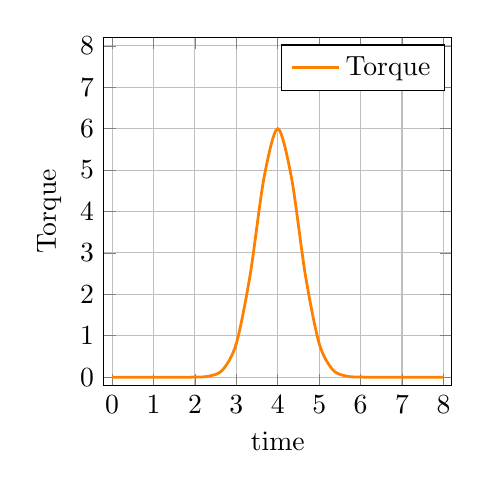
\begin{tikzpicture}
    \begin{axis}[
      xlabel={time},
      ylabel={Torque},
      width=8cm,
      height=6cm,
      axis equal image,
      xtick distance=1,
      ytick distance=1,
      grid=major,
      grid style={gray!50},
      grid=both,
      xmin=-0.2,
      xmax=8.2,
      ymin=-0.2,
      ymax=8.2
    ]
    \addplot[color=orange, smooth, line width=1pt, domain=0:8] {6*exp(-((x-4)^2)/(2*0.5^2))};
    \addlegendentry{Torque}
  \end{axis}
  \end{tikzpicture}

\end{Exercise}

\begin{Answer}[ref={ex:ang_imp}]
As we can see, each unit square is equivalent to $1 \,\ \mathrm{torque}\cdot \mathrm{time}$. Counting the partial and full squares on $t=[2,6]$, we get approximately 8 unit squares. This comes from the (approximately whole) 4 squares under $y=2$, combining all squares from $y=[2,4]$ to form 2 squares, and the additional partial area forming approximately another 2 squares, resulting in an angular impulse of approximately $8 \text{ N}\cdot \text{m} \cdot \text{s}$. 

Counting squares is a first step toward \emph{integration}, a calculus method for finding areas under curves exactly. When you learn it, you will find that the exact area here is about $7.52 \text{ N}\cdot \text{m} \cdot \text{s}$, pretty close to our estimate.
\end{Answer}
\subsection{Work done by Torque}\index{work!by torque}
Recall that work is a change in energy. Torque also does work when it causes rotation. For a constant torque acting on point mass through an angular displacement $\Delta \theta$ the work done is
\begin{equation}
W = Fr\,\Delta\theta = \tau \Delta \theta
\label{eq:work_rot}
\end{equation}

This comes from the fact that linear work is defined as $W = F \Delta x$, and the arc length of a circle is defined as $s = r \theta$. Thus, we can substitute $r \theta$ for $\Delta x$ in the linear work equation to get the rotational work equation.

\section{Summary}
Here is a summary of linear quantities in physics, and their now introduced rotational components. You will refer to it often, so keep it handy.
\begin{table}[H]
\centering
\renewcommand{\arraystretch}{1.5}
\caption{Correspondence Between Linear and Rotational Motion}
\label{tab:linear_rotational_analogy}
\begin{tabular}{|c|c|}
\hline
\textbf{Linear Motion} & \textbf{Rotational Motion} \\
\hline
Position $x$ & Angle $\theta$ \\
\hline
Velocity $v$ & Angular velocity $\omega$ \\
\hline
Acceleration $a$ & Angular acceleration $\alpha$ \\
\hline
Mass $m$ & Moment of inertia $I$ \\
\hline
Force $F$ & Torque $\tau$ \\
\hline
Momentum $p = mv$ & Angular momentum $L = I\omega$ \\
\hline
$F = \dfrac{\Delta p}{\Delta t}$ & $\tau = \dfrac{\Delta L}{\Delta t}$ \\
\hline
Work $W = F \Delta x$ & Work $W = \tau \Delta \theta$ \\
\hline
Kinetic Energy $\tfrac{1}{2}mv^2$ & Rotational KE $\tfrac{1}{2}I\omega^2$ \\
\hline
Power $P = Fv$ & Power $P = \tau \omega$ \\
\hline
\end{tabular}
\end{table}
